\documentclass[10pt,a4paper]{report}
\usepackage[utf8]{inputenc}
\usepackage{amsmath}
\usepackage{amsfonts}
\usepackage{amssymb}
\author{Jacek Czyrnek, Adam Koleszar, Marion Le Guével, Mihaly Lengyel
•
}
\usepackage{graphicx}
\graphicspath{{/home/pandachan/Documents/cours/Group_project/}}
\title{Group project report}
\begin{document}

\chapter{Introduction}


\chapter{Technical review}


\chapter{Requirements specifications}
	\subsection{Usecases}
This project handle login as sessions. Therefore each session (a set of iterations) is a new user with a new password.  However, all these "users" are of the same type and have the same functionnalities : \\
%\includegraphics[scale=0.4]{Usecase_group-project.png}
Mainly, the purpose of this software is to solve an equation with different given parameters and to display the result graphically.
	\subsection{Functional and non functional requirements}
On the previous usecase, different functionalities are written. This subsection will detailed those functionalities into functional and non functional requirements.
		\subsubsection{Functional requirements}
\begin{tabular}{|c|c|}
\hline 
\textbf{ID} & \textbf{Requirement} \\ 
\hline 
1 & To log into a session \\ 
\hline 
2 & To create a new session \\ 
\hline 
3 & As logged in : To enter new inputs \\ 
\hline
4 & As logged in : To start or stop iterating on the equation (exchange of data with the cluster) \\ 
\hline
5 & As logged in : To display the result of the iterations in real time on a graph \\ 
\hline
6 & As logged in : To display the result of the iterations in real time as a wing modeling \\ 
\hline
7 & As logged in : To download the log file (exchange of data with the cluster)\\ 
\hline
8 & As logged in : To logout from a session \\ 
\hline
\end{tabular} 
		\subsubsection{Non-functional requirements}
\begin{tabular}{|c|c|}
\hline 
\textbf{Type} & \textbf{Requirement} \\ 
\hline 
Security & To log into a session with a password so only people having those\\
 & information can access to it\\ 
\hline 
Reliability & To have a recovery system to access previous steps of a session \\ 
\hline 
Speed & To use a cluster for solving the equation \\ 
\hline
\end{tabular} 
	\subsection{Further information}
An example has been given for the software user interface. With the functionalities required, the final product should have two "pages", one for the connexion or creation of a session, and another one once logged in a session, as the mockups below:\\
%\includegraphics[scale=0.4]{group_project_mockups.png}

\pagebreak
\section{System design}
\subsection{Component diagram}
We began the design process by dividing the system into bigger modules and designing the interfaces between them to conduce parallel work. We split the software into 4 bigger modules and assigned one to each team member:\\
\begin{enumerate}
\item Database \& Session: Marion Le Guével
\item Atlas Connector: Ádám Koleszár
\item GUI: Jacek Czyrnek
\item Wing Visualizer: Mihály Lengyel
\end{enumerate}
The following diagram shows the components of the system and the interfaces they interact through.
\begin{figure}[h!]
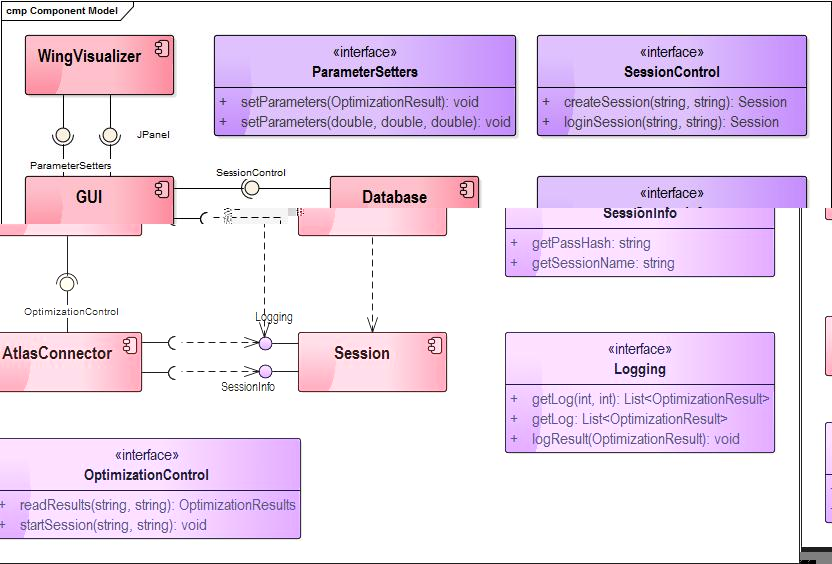
\includegraphics[width=\textwidth]{CompModel.jpg}
\caption{Component diagram}
\end{figure}
\pagebreak

\subsection{Class diagram}
In the following diagram you can see, that the classes in the implemented system are simple reflections of the component design above.
\begin{figure}[h!]
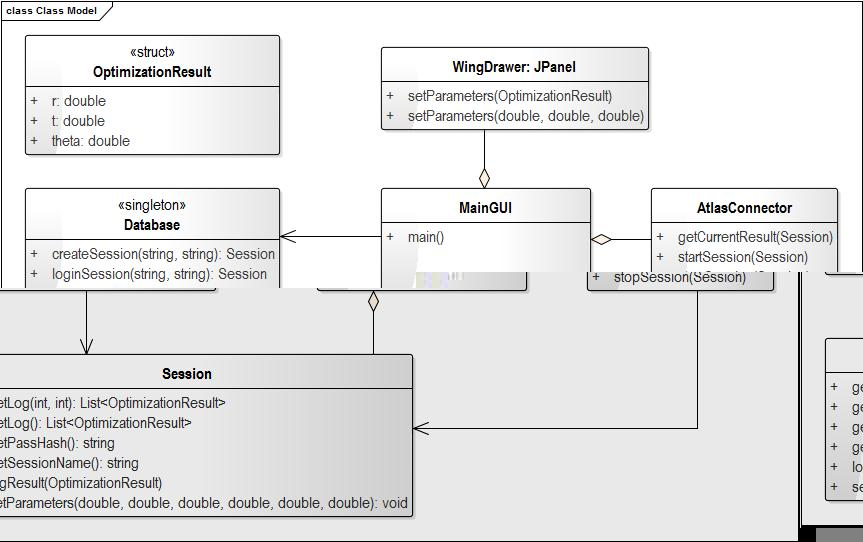
\includegraphics[width=\textwidth]{ClassModel.jpg}
\caption{Class diagram}
\end{figure}
\pagebreak
\subsection{Sequence diagram}
To complement the static diagrams above here we provide a diagram to show the dynamic behaviour of the system. This is not an exact sequence diagram but it shows the flow of data through the system.
\begin{figure}[h!]
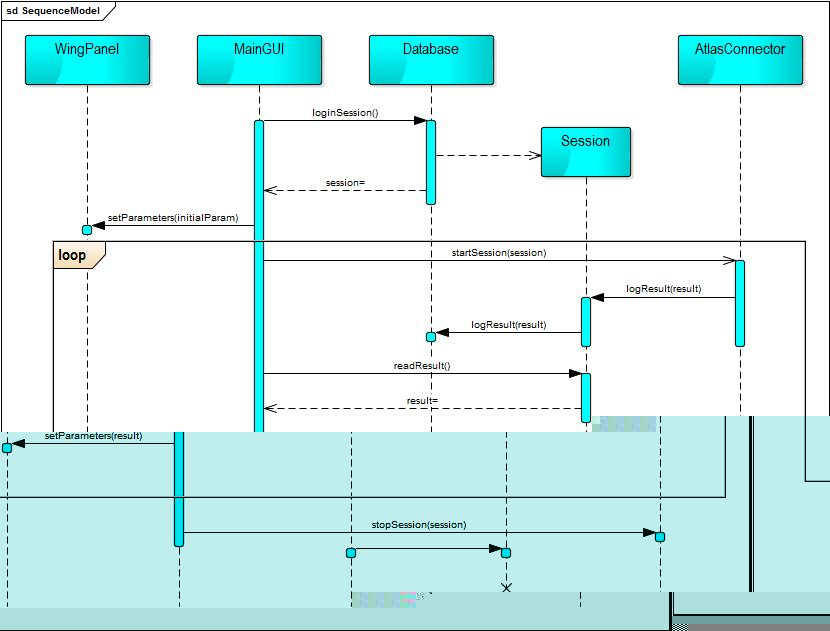
\includegraphics[width=\textwidth]{SequenceModel.jpg}
\caption{Sequence diagram}
\end{figure}

\end{document}